\section{设计方案}

\subsection{总体设计思路}

\begin{figure}[H]
  \centering
  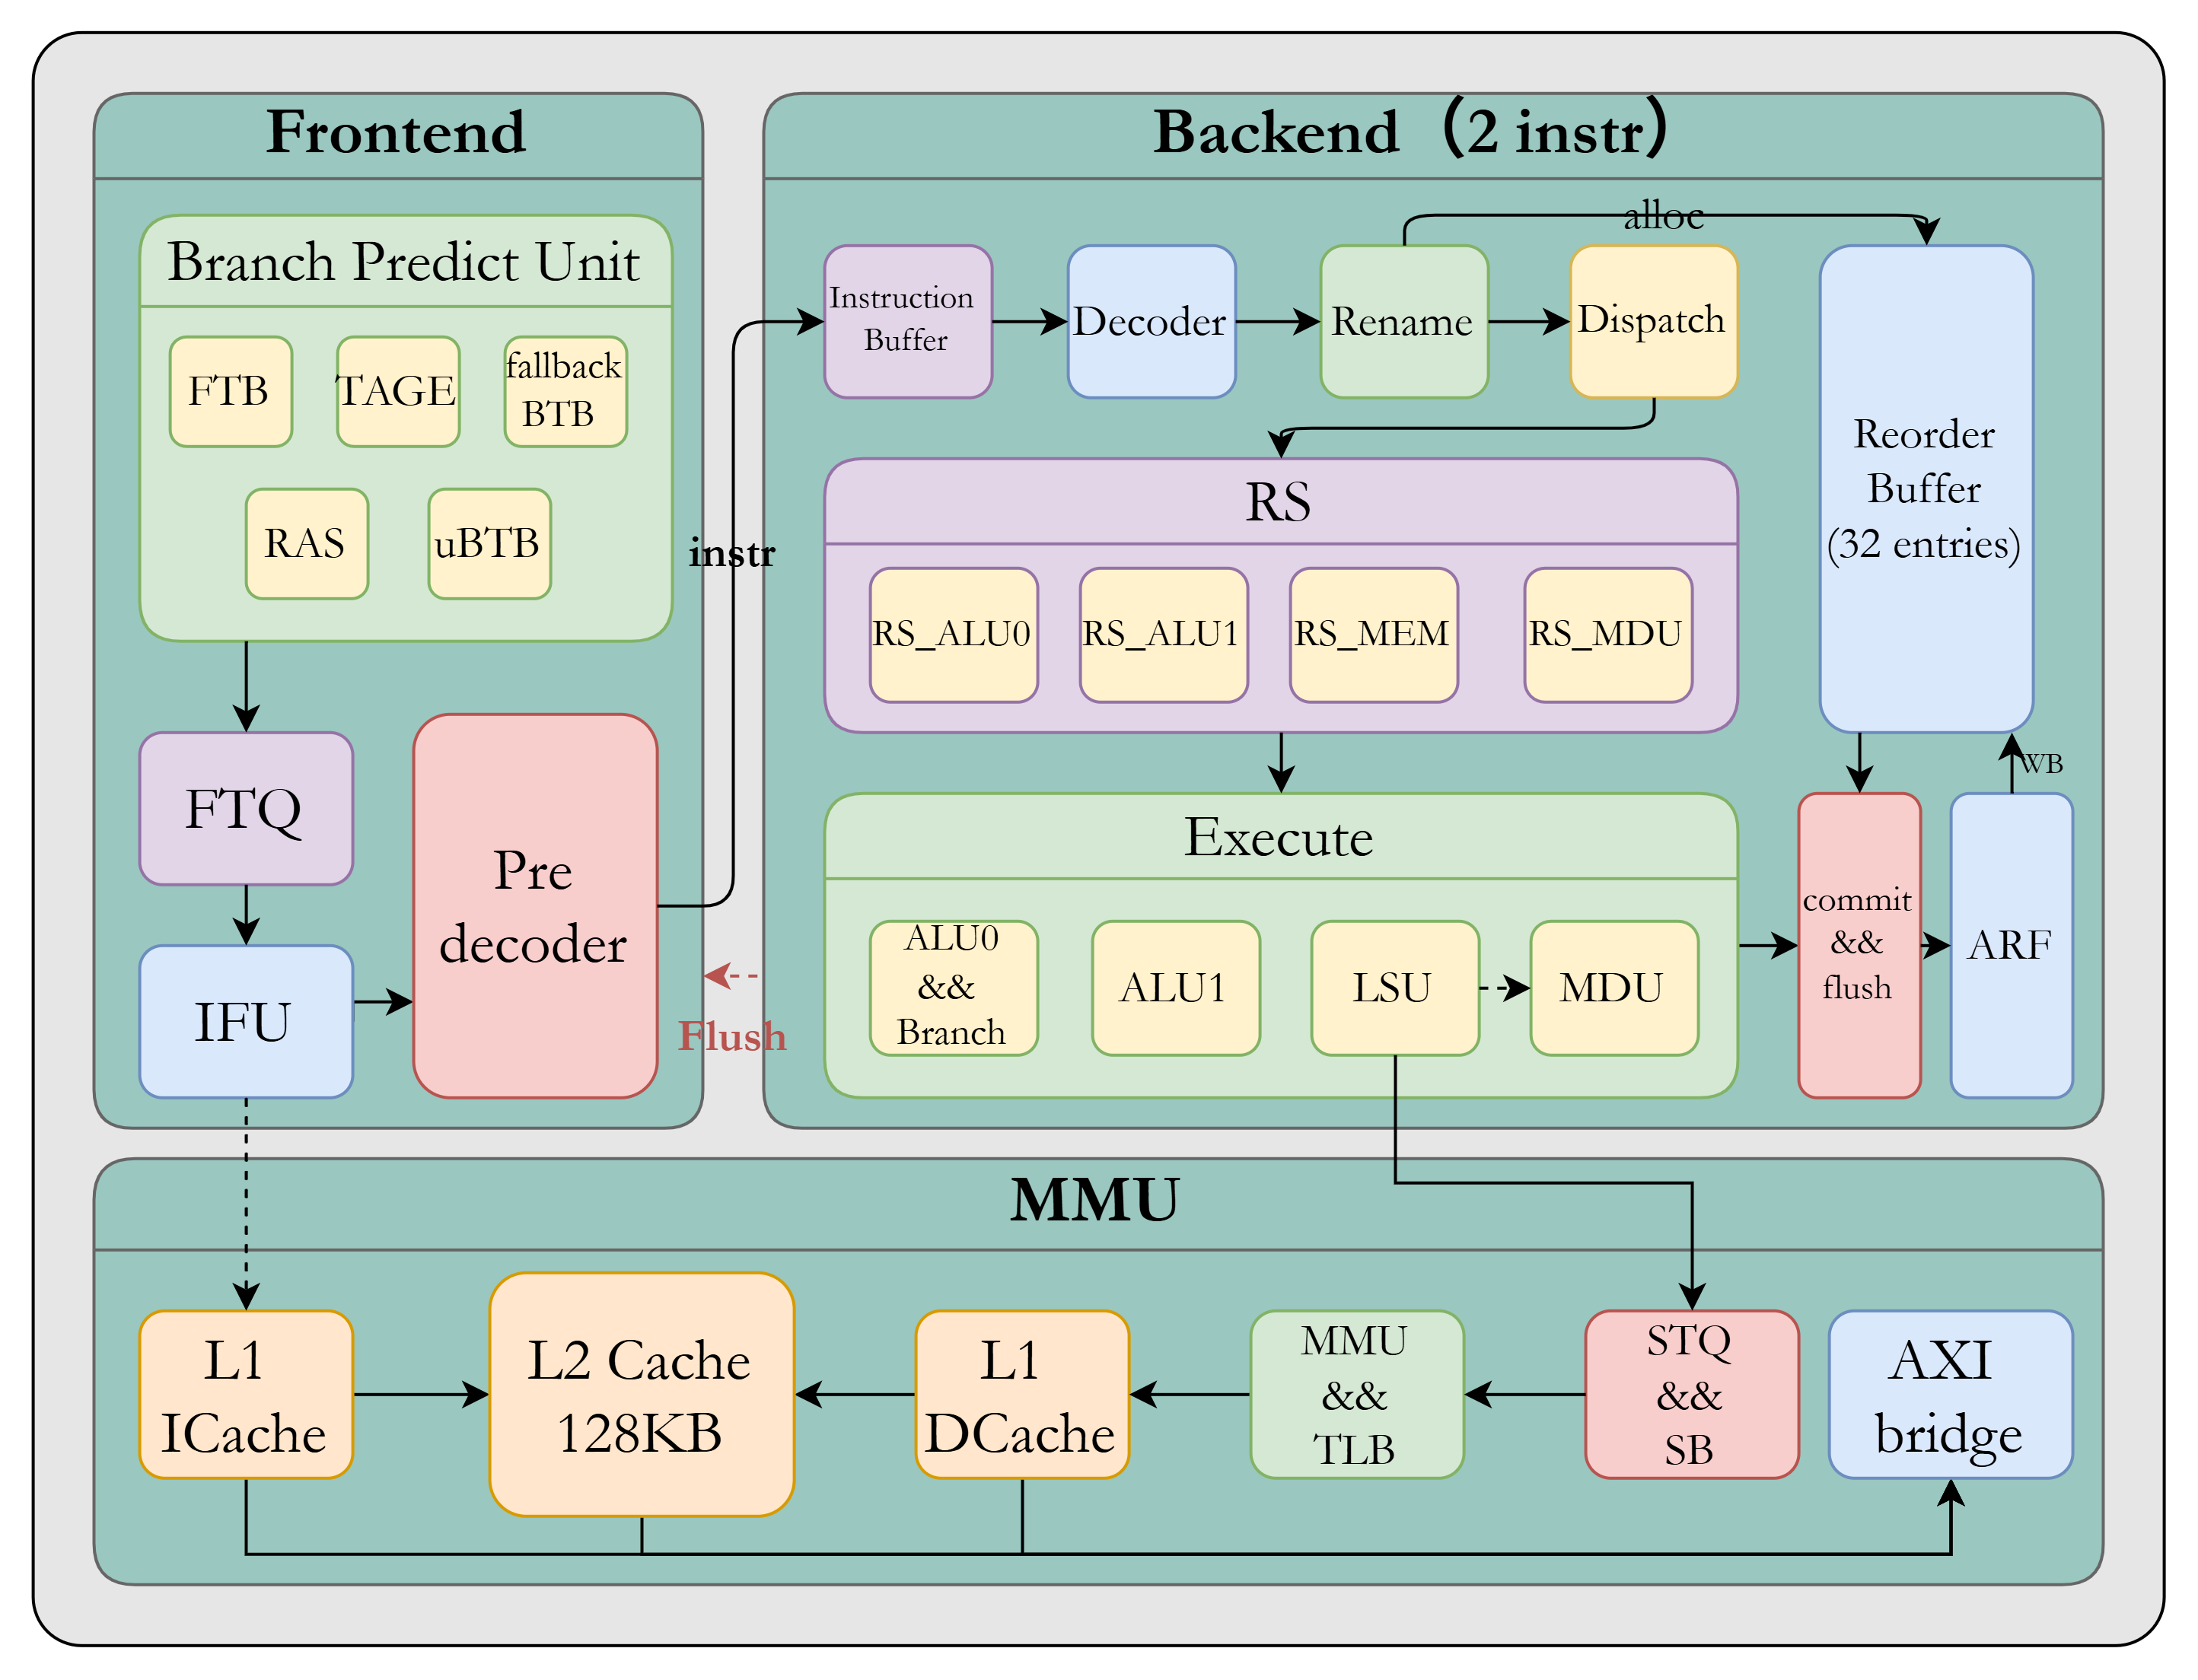
\includegraphics[width=0.95\textwidth]{figure/mycpu_arch.png}
  \caption{CPU 设计架构图}
  \label{fig:cpuarch}
\end{figure}

意味核采用前后端解耦的乱序结构。前端由分支预测器、FTQ、IFU、ICache 和 IB 组成，以最多 4 条指令的基本块推进；后端由译码、重命名、分发、异构保留站、三路 ALU、LSU、MDU、ROB 与提交控制组成。ROB 编号直接作为重命名标签，结果保存在 ROB 中，已提交的 ARF 是全局恢复后的权威状态，不设置独立 PRF 与 freelist。

处理器以 2 宽作为稳定基线：常规路径每拍处理两条指令；当 IB 中第三条指令满足资源与类型约束时，可机会式进入第三译码、重命名和分发通路，三条均为 ALU 类时可使用三路整数执行单元。提交级通常退休 2 条指令，在队首两条正常提交且下一对简单指令均已完成、无例外和串行副作用时，可启用受限四退休快路径。

指令执行过程如下：
\begin{enumerate}
  \item \textbf{预测与取指}：BPU 生成最多 4 条指令的预测块，FTQ 保存预测元数据，IFU 经 MMU 与 ICache 取回指令并写入 IB；
  \item \textbf{译码与重命名}：生成操作类型、立即数、特权和例外信息，查询 RAT/ARF/ROB 获得源操作数，以 ROB 编号建立寄存器依赖；
  \item \textbf{分发与发射}：按 ALU、MEM、MDU 三类路由到异构保留站，在操作数和功能单元就绪后发射；
  \item \textbf{执行与写回}：ALU、LSU 和 MDU 完成运算，将结果、分支结果或例外信息写回 ROB；
  \item \textbf{按序提交}：提交级更新 ARF、CSR、TLB、LLBit 与 Store Buffer，并统一处理分支误预测、例外、\texttt{ertn} 和缓存维护引起的重取。
\end{enumerate}

\begin{table}[H]
\centering
\caption{主要结构容量}
\label{tab:capacity}
\small
\begin{tabularx}{\textwidth}{>{\raggedright\arraybackslash}p{3.3cm}X}
\toprule
结构 & 规格 \\
\midrule
取指与后端宽度 & 每块最多 4 条取指；2 宽基线；机会式三宽译码、重命名与分发；受限四退休 \\
ROB & 32 项，奇偶双体组织 \\
IB / FTQ & 16 项 / 16 项 \\
保留站 & RS\_ALU $3\times5$ 项；RS\_MEM 8 项；RS\_MDU 2 项 \\
STQ / Store Buffer & 16 项 / 8 项 \\
L1 Cache & ICache、DCache 各 16\,KiB，4 路$\times$128 组$\times$32\,B，VIPT \\
L2 Cache & 128\,KiB，2 路$\times$2048 组$\times$32\,B，写回式 \\
TLB & 主 TLB 32 项、双查询口；I/D 微 TLB 各 8 项 \\
BPU & uBTB 32 项；fallback BTB 128 项；FTB $4\times2048$；TAGE 8K$+4\times2$K；局部预测器；RAS 32 双栈 \\
\bottomrule
\end{tabularx}
\end{table}

\subsubsection{指令实现}

处理器实现表~\ref{tab:inst} 所列 LA32R 整数与特权指令子集。\texttt{preld} 被识别为合法指令并以无执行副作用的方式退休；\texttt{ibar}/\texttt{dbar} 在提交级等待 Store Buffer 排空后触发重取，从而保证屏障之前的访存已经对系统可见。当前实现不包含浮点与向量执行单元。

\begin{table}[H]
\centering
\caption{指令实现}
\label{tab:inst}
\scriptsize
\begin{tabularx}{\textwidth}{>{\raggedright\arraybackslash}p{2.7cm}X}
\toprule
指令类型 & 指令名称 \\
\midrule
算术与逻辑 & \texttt{add.w}, \texttt{sub.w}, \texttt{addi.w}, \texttt{slt}, \texttt{sltu}, \texttt{slti}, \texttt{sltui}, \texttt{lu12i.w}, \texttt{pcaddu12i}, \texttt{pcaddi}, \texttt{and}, \texttt{or}, \texttt{nor}, \texttt{xor}, \texttt{andn}, \texttt{orn}, \texttt{andi}, \texttt{ori}, \texttt{xori} \\
移位 & \texttt{sll.w}, \texttt{srl.w}, \texttt{sra.w}, \texttt{slli.w}, \texttt{srli.w}, \texttt{srai.w} \\
乘除 & \texttt{mul.w}, \texttt{mulh.w}, \texttt{mulh.wu}, \texttt{div.w}, \texttt{div.wu}, \texttt{mod.w}, \texttt{mod.wu} \\
分支跳转 & \texttt{beq}, \texttt{bne}, \texttt{blt}, \texttt{bltu}, \texttt{bge}, \texttt{bgeu}, \texttt{b}, \texttt{bl}, \texttt{jirl} \\
普通访存 & \texttt{ld.b}, \texttt{ld.bu}, \texttt{ld.h}, \texttt{ld.hu}, \texttt{ld.w}, \texttt{st.b}, \texttt{st.h}, \texttt{st.w} \\
原子访存 & \texttt{ll.w}, \texttt{sc.w} \\
屏障与预取 & \texttt{ibar}, \texttt{dbar}, \texttt{preld} \\
特权与 TLB & \texttt{csrrd}, \texttt{csrwr}, \texttt{csrxchg}, \texttt{tlbsrch}, \texttt{tlbrd}, \texttt{tlbwr}, \texttt{tlbfill}, \texttt{invtlb}, \texttt{cacop}, \texttt{ertn}, \texttt{idle} \\
系统与计时器 & \texttt{syscall}, \texttt{break}, \texttt{rdcntid}, \texttt{rdcntvl.w}, \texttt{rdcntvh.w}, \texttt{cpucfg} \\
\bottomrule
\end{tabularx}
\end{table}

\subsubsection{CSR 实现}

CSR 模块保存处理器模式、例外、中断、计时器、TLB 和直接映射窗口状态。未实现编号的 CSR 读返回 0、写忽略；TICLR、SAVE0--3、TID 等低风险寄存器采用快速写路径，其他会改变执行环境的 CSR 写在提交级串行完成。

\begin{table}[H]
\centering
\caption{主要 CSR}
\label{tab:csr}
\scriptsize
\begin{tabularx}{\textwidth}{cXlcXl}
\toprule
地址 & 含义 & 名称 & 地址 & 含义 & 名称 \\
\midrule
0x0 & 当前模式信息 & CRMD & 0x30--33 & 数据保存 & SAVE0--3 \\
0x1 & 例外前模式信息 & PRMD & 0x40 & 定时器编号 & TID \\
0x2 & 扩展组件使能 & EUEN & 0x41 & 定时器配置 & TCFG \\
0x4 & 例外配置 & ECFG & 0x42 & 定时器值 & TVAL \\
0x5 & 例外状态 & ESTAT & 0x44 & 定时中断清除 & TICLR \\
0x6 & 例外返回地址 & ERA & 0x60 & LLBit 控制 & LLBCTL \\
0x7 & 出错虚地址 & BADV & 0x88 & TLB 重填入口 & TLBRENTRY \\
0xC & 例外入口地址 & EENTRY & 0x180--181 & 直接映射窗口 & DMW0--1 \\
0x10 & TLB 索引 & TLBIDX & 0x18 & 地址空间编号 & ASID \\
0x11 & TLB 表项高位 & TLBEHI & 0x19--1B & 页目录基址 & PGDL/H/D \\
0x12--13 & TLB 表项低位 & TLBELO0/1 & 0x20 & 处理器编号 & CPUID \\
\bottomrule
\end{tabularx}
\end{table}

\subsubsection{例外与中断}

例外信息随指令在流水线中传递，最终在提交级按优先级编码并更新 CSR，以保证精确例外。8 路外部硬中断接入 ESTAT.IS[9:2]，定时器中断接入 ESTAT.IS[11]。\texttt{idle} 退休后停止取指，直至可响应中断到来。

\begin{table}[H]
\centering
\caption{例外与中断类型}
\label{tab:excp}
\small
\begin{tabular}{cccc}
\toprule
Ecode & Esubcode & 代号 & 类型 \\
\midrule
0x0 & 0 & INT & 中断 \\
0x1 & 0 & PIL & Load 页无效 \\
0x2 & 0 & PIS & Store 页无效 \\
0x3 & 0 & PIF & 取指页无效 \\
0x4 & 0 & PME & 页修改 \\
0x7 & 0 & PPI & 页特权等级不合规 \\
0x8 & 0 & ADEF & 取指地址错误 \\
0x8 & 1 & ADEM & 访存地址错误 \\
0x9 & 0 & ALE & 地址非对齐 \\
0xB & 0 & SYS & 系统调用 \\
0xC & 0 & BRK & 断点 \\
0xD & 0 & INE & 指令不存在 \\
0xE & 0 & IPE & 指令特权等级错误 \\
0x3F & 0 & TLBR & TLB 重填 \\
\bottomrule
\end{tabular}
\end{table}

\subsubsection{地址翻译模式}

CRMD.DA$=1$、PG$=0$ 时采用直接地址；DA$=0$、PG$=1$ 时先匹配 DMW0/DMW1，未命中窗口则查询 TLB。TLB 表项同时给出物理页号、页大小、有效位、脏位、特权等级和存储访问类型，相关例外随取指或访存指令进入 ROB，并在提交级处理。
